\documentclass[journal,12pt,twocolumn]{IEEEtran}
\usepackage{amsmath,amssymb,amsfonts,amsthm}
\usepackage{txfonts}
\usepackage{tkz-euclide}
\usepackage{listings}
\usepackage{gvv}
\usepackage[latin1]{inputenc}
\usepackage{array}
\usepackage{pgf}
\usepackage{lmodern}

\begin{document}
\bibliographystyle{IEEEtran}

\title{GATE 2022[EE]-19}
\author{EE23BTECH11066 - Yakkala Amarnath Karthik}
\maketitle
\bibliographystyle{IEEEtran}

\textbf{Question:}\\ \\
The open loop transfer function of a unity gain negative feedback system is given by $G\brak{s}= \frac{k}{s^2 +4s-5}$. The range of k for which the system is stable,is\hfill(GATE EE 2022)\\ \\

\textbf{Solution:}\\ 
\begin{table}[ht]
  \begin{tabular}{|c|c|c|}
    \hline
    \textbf{Variable} & \textbf{Description} & \textbf{value}\\
    \hline
    $G\brak{s}$ & Open loop transfer function & $\frac{k}{s^2 +4s-5}$\\
   \hline
    1+G$\brak{s}$ & Characteristic equation & 0 \\
    \hline
    \end{tabular}
  \caption{A Table with input parameters}
  \label{tab:gate2022ee19}
\end{table}
\\
 from Table\ref{tab:gate2022ee19}\\
Characteristic equation:
\begin{align}
    1+G\brak{s}=0\\
    \implies 1+\frac{k}{s^2 +4s-5}=0\\
    \implies s^2+4s+\brak{k-5}=0
\end{align}
By routh table analysis, for a stable system:
\begin{align}
    k-5>0\\
    \implies k>5
\end{align}


\begin{figure}[ht]
    \centering
    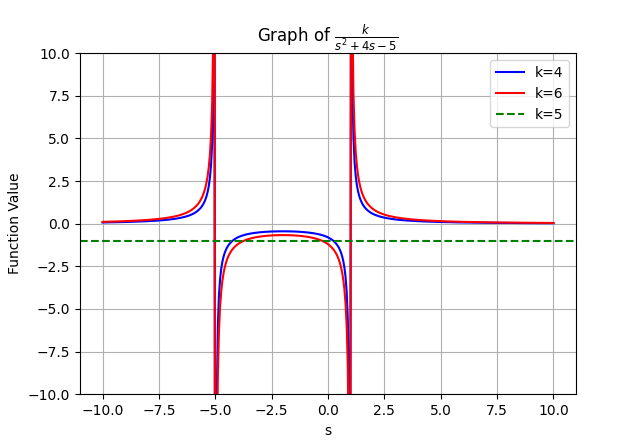
\includegraphics[width=0.45\textwidth]{figs/gate2022.png}
    \caption{Graph showing $k<5,k=5,k>5$}
\end{figure}
\end{document}
